\begin{surferIntroPage}{Veiledning}{tutorial_koord1}{Første skritt med SURFER}
 Dette programmet heter SURFER. Når du leser ordet, tenker du kanskje på vann, sol og bølger. 
 Navnet til programmet kommer fra det engelske ordet surface, som betyr {\it flate}. 
\\
Med SURFER kan du visualisere flater, nærmere bestemt algebraiske flater. Hva det betyr og 
hva algebraiske flater er, kan du lese mer om i denne innføringen. Trykk på figurene til 
høyre for å se gjennom kapitlene.\\

SURFER er en del av vandreutstillingen IMAGINARY, som startet opp som en del av Matematikkåret
 2008 i Tyskland. Bak utstillingen står det internasjonalt kjente Mathematisches Forschungsinstitut 
 Oberwolfach i Schwarzwald. Hver uke holder instituttet åpne møter om aktuell matematisk forskning.
 Disse møtene er viktige for utveksling av informasjon mellom forskere over hele verden.\\
 
\vspace{0.2cm} \hspace{3.5cm}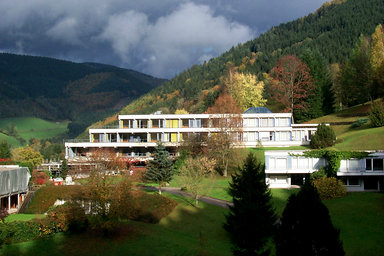
\includegraphics[width=3cm]{./../../common/images/photo_mfo.jpg}\\
Du kan laste ned programmet SURFER gratis på hjemmesiden: \\
\begin{centering}
www.imaginary-exhibition.com\\
\end{centering}
 \vspace{0.2cm}
Til høyre kan du velge en av de matematiske innføringene, som starter med sitrus-flaten.
 Til venstre kan du hoppe til de andre galleriene, for eksempel galleriet med fantasiflater.
\end{surferIntroPage}
